% Using Free and Open Source Solutions in Geospatial Science Education
% This work by Vaclav Petras is licensed under
% a Creative Commons Attribution-ShareAlike 4.0 International License.

\documentclass[xcolor={dvipsnames,usenames},beamer,aspectratio=43]{beamer}
% ,handout,notes=show

\makeatletter
\def\beamer@framenotesbegin{% at beginning of slide
  \gdef\beamer@noteitems{}%
  \gdef\beamer@notes{{}}% used to be totally empty.
}
\makeatother

\usepackage{textcomp}
\usepackage[utf8]{inputenc}
\usepackage[american]{babel}
\usepackage{graphicx}
\usepackage{url}
\usepackage{amssymb}

\usepackage{alltt}

\usepackage{tikz}
\usetikzlibrary{arrows,shapes,spy,calc}

\tikzstyle{every picture}+=[remember picture]
\tikzstyle{na} = [baseline=-.5ex]

% don't count bacup slides
\newcommand{\backupbegin}{
   \newcounter{finalframe}
   \setcounter{finalframe}{\value{framenumber}}
}
\newcommand{\backupend}{
   \setcounter{framenumber}{\value{finalframe}}
}

% frames have to be fragile
\newif\ifnotes
% \input{tmpnotessettings}
% \notestrue


\ifnotes
\setbeamertemplate{note page}[plain]
% \setbeamertemplate{note page}[compress]
\setbeamerfont{note page}{size=\large}
% \setbeameroption{show only notes}
\setbeameroption{show notes}
\usepackage{pgfpages}
\pgfpagesuselayout{2 on 1}[a4paper,border shrink=5mm]%
\else
%\setbeameroption{hide notes}
\fi
%\notesfalse

\usepackage[absolute,overlay]{textpos}

\usepackage{listings}


% \usetheme{Warsaw}
\usetheme{Madrid}
% \usetheme{Frankfurt}
% \useoutertheme{infolines}
\usecolortheme[named=MidnightBlue]{structure}
% \usecolortheme[named=PineGreen]{structure}
\setbeamertemplate{navigation symbols}{}

\setbeamertemplate{itemize items}[default]
\setbeamertemplate{enumerate items}[default]
% \useinnertheme{rectangles}
\setbeamertemplate{blocks}[default]


%%%%%%%%%%%%%%%%%%%%%%%%%%%%%%%%%%%%%%%%%%%%%%%%%%%%%%%%%%%%%%%%%%%%
%%%%%%%%%%%%%%%%%%%%%%%%%%%%%%%%%%%%%%%%%%%%%%%%%%%%%%%%%%%%%%%%%%%%

% \newcommand{\n}[1]{$^{\color{gray}{\mbox{\tiny#1}}}$}
\newcommand{\n}[1]{$^{\textcolor{gray}{\mbox{\tiny #1}}}$}

%%%%%%%%%%%%%%%%%%%%%%%%%%%%%%%%%%%%%%%%%%%%%%%%%%%%%%%%%%%%%%%%%%%%%%%%%%%%%%%
\newcommand{\gmodule}[1]{\href{http://grass.osgeo.org/grass71/manuals/#1.html}{\emph{#1}}}
\newcommand{\amodule}[1]{\href{http://grass.osgeo.org/grass70/manuals/addons/#1.html}{\emph{#1}}}
\newcommand{\module}[1]{\emph{#1}}
\newcommand{\grasslink}{\href{http://grass.osgeo.org/}{GRASS GIS}}

%%%%%%%%%%%%%%%%%%%%%%%%%%%%%%%%%%%%%%%%%%%%%%%%%%%%%%%%%%%%%%%%%%%%
%%%%%%%%%%%%%%%%%%%%%%%%%%%%%%%%%%%%%%%%%%%%%%%%%%%%%%%%%%%%%%%%%%%%

\title[Point clouds in GRASS GIS]{Processing UAV and lidar point clouds in GRASS GIS}
\subtitle{XXIII ISPRS Congress, Prague 2016}
%\pdforstring{}{}

\author[Vaclav Petras]
{Vaclav Petras (Vashek)\\
{
\scriptsize
Anna Petrasova,
Justyna Jeziorska,
Helena Mitasova
}
}

\institute[NC State University]
{%
Center for Geospatial Analytics

\bigskip

\includegraphics[width=0.3\textwidth]{logos/ncstate}
}

\date{July, 2016}

\setbeamercovered{transparent}

\hypersetup{%
 pdfauthor={Vaclav Petras},%
 pdfsubject={Point clouds and GRASS GIS talk at ISPRS 2016},%
 pdfkeywords={3D rasters} {decimation} {sampling} {binning}
   {LAS} {PDAL} {PCL} {Kinect}
   {v.in.lidar} {r.in.lidar} {r.in.kinect} {libLAS}
   {geospatial modeling}
   {free software} {open source} {open science}
}

\usepackage{tipa}
\newcommand{\pron}[2]{#1 [#2]}


%%%%%%%%%%%%%%%%%%%%%%%%%%%%%%%%%%%%%%%%%%%%%%%%%%%%%%%%%%%%%%%%%%%%
% when images are placed in these directories, we don't have to specify the directory
% just the filename
\graphicspath{{img/}{figures/}{images/}}


%%%%%%%%%%%%%%%%%%%%%%%%%%%%%%%%%%%%%%%%%%%%%%%%%%%%%%%%%%%%%%%%%%%%
%%%%%%%%%%%%%%%%%%%%%%%%%%%%%%%%%%%%%%%%%%%%%%%%%%%%%%%%%%%%%%%%%%%%
%%%%%%%%%%%%%%%%%%%%%%%%%%%%%%%%%%%%%%%%%%%%%%%%%%%%%%%%%%%%%%%%%%%%
%%%%%%%%%%%%%%%%%%%%%%%%%%%%%%%%%%%%%%%%%%%%%%%%%%%%%%%%%%%%%%%%%%%%
\begin{document}

\newcommand{\logowidth}{1.0em}
\newcommand{\logospace}{\hspace{0.2em}}
\newcommand{\includecclogo}[1]{\includegraphics[width=\logowidth]{./images/logos/#1}}

%%%%%%%%%%%%%%%%%%%%%%%%%%%%%%%%%%%%%%%%%%%%%%%%%%%%%%%%%%%%%%%%%%%%
\frame{
\titlepage
\begin{center}
\vspace{-3ex}
\href{http://creativecommons.org/licenses/by-sa/4.0/}{
\includecclogo{cc}
\logospace
\includecclogo{by}
\logospace
\includecclogo{sa}
}
\\
\footnotesize
available at\\
\href{http://wenzeslaus.github.io/grass-lidar-talks/}{\texttt{wenzeslaus.github.io/grass-lidar-talks}}
\end{center}
}


%%%%%%%%%%%%%%%%%%%%%%%%%%%%%%%%%%%%%%%%%%%%%%%%%%%%%%%%%%%%%%%%%%%%%
\begin{frame}{Providing algorithms to the community}

\begin{itemize}
  \item new landform recognition approach -- geomorphons
\end{itemize}

\begin{columns}
\begin{column}{0.4\textwidth}

\begin{itemize}
  % Adam Mickiewicz University and University of Cincinnati
  \item by Jasiewicz and Stepinski
    {\tiny from AMU, Poland and University of Cincinnati, USA}
  \item not just a paper
    {\tiny Geomorphology, 2013}
  \item not just a code
    \\{\tiny at some webpage}
  \item \amodule{r.geomorphon}
    \\{\tiny module in GRASS GIS addons repository}
\end{itemize}

\end{column}
\begin{column}{0.58\textwidth}

\begin{center}
  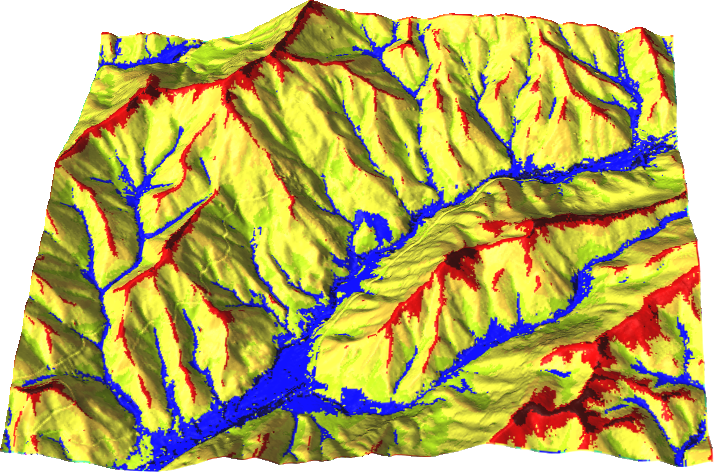
\includegraphics[width=\textwidth]{vis/geomorphon_3d}
\end{center}

\end{column}
\end{columns}

\end{frame}


%%%%%%%%%%%%%%%%%%%%%%%%%%%%%%%%%%%%%%%%%%%%%%%%%%%%%%%%%%%%%%%%%%%%%
\begin{frame}{GRASS GIS}

\begin{columns}
\begin{column}{0.6\textwidth}

\begin{itemize}
  \item all in one
  \begin{itemize}
   \item hydrology modeling, image segmentation, point clustering, \ldots
  \end{itemize}
  \item driven by needs of users
  \begin{itemize}
   \item direct access to development process
  \end{itemize}
  \item from small laptops to supercomputers
  \begin{itemize}
   \item Raspberry Pi, Windows, Mac, GNU/Linux, FreeBSD, IBM~AIX
  \end{itemize}
  \item learn now, use forever
  \begin{itemize}
    \item over 30 years of development and interface refinement
  \end{itemize}
  \item used by
  \begin{itemize}
    \item US Oak Ridge National Laboratory, Edmund Mach Foundation, JRC, \ldots
  \end{itemize}
\end{itemize}

\end{column}
\begin{column}{0.3\textwidth}

\begin{center}
  
\includegraphics[width=\textwidth]{logos/grass_gis}
\end{center}

\textcolor{gray}{
\footnotesize
latest release 7.0.4 \\May~1,~2016
}

\end{column}
\end{columns}

\end{frame}


%%%%%%%%%%%%%%%%%%%%%%%%%%%%%%%%%%%%%%%%%%%%%%%%%%%%%%%%%%%%%%%%%%%%%
\begin{frame}{GUI}

\begin{center}
  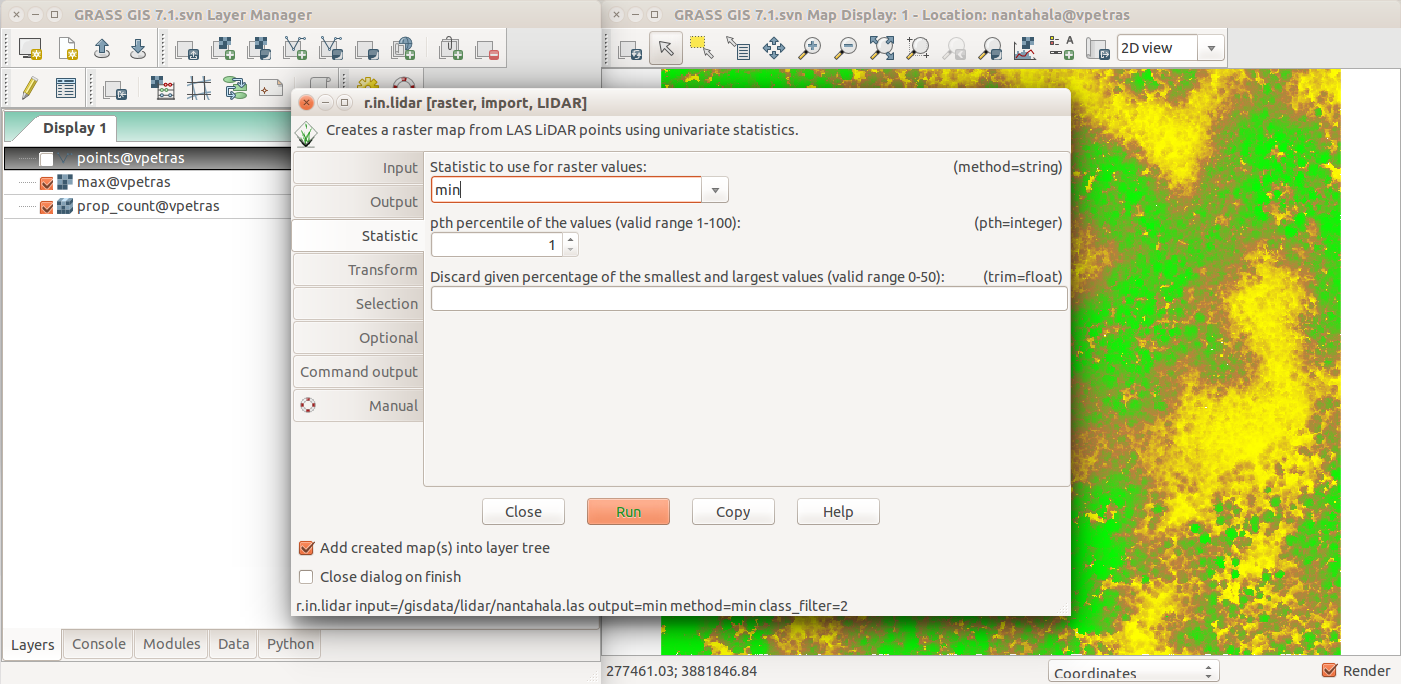
\includegraphics[width=0.9\textwidth]{grass/r_in_lidar_gui}
\end{center}

\end{frame}


%%%%%%%%%%%%%%%%%%%%%%%%%%%%%%%%%%%%%%%%%%%%%%%%%%%%%%%%%%%%%%%%%%%%%
\begin{frame}{Python and command line interfaces}

\definecolor{mod}{RGB}{7,96,143}
\definecolor{opt}{RGB}{239,84,18}
\definecolor{flg}{RGB}{239,84,18}
\definecolor{txt}{RGB}{45,146,45}
\definecolor{bash}{RGB}{200,200,200}
\definecolor{import}{RGB}{200,200,200}

\Large

Command Line:

\LARGE

\begin{alltt}
\textcolor{mod}{r.in.lidar} \textcolor{opt}{input}=\textcolor{txt}{points.las} \textcolor{bash}{\char`\\}
\\%
\newlength{\shindent}
\settowidth{\shindent}{r.in.lidar~}
\rule{\shindent}{0pt}%
\textcolor{opt}{output}=\textcolor{txt}{elevation} -\textcolor{flg}{e}
\end{alltt}

\Large

Python:

% \char`_ is to get same underscore as in \verb

\LARGE

\begin{alltt}
\textcolor{import}{from grass.script import run\char`_command}
\\
run\char`_command('\textcolor{mod}{r.in.lidar}',
%
\newlength{\pyindent}%
\settowidth{\pyindent}{run\_command(}%
\\%
\rule{\pyindent}{0pt}\,%
\textcolor{opt}{input}="\textcolor{txt}{points.las}",
\\%
\rule{\pyindent}{0pt}\,%
\textcolor{opt}{output}="\textcolor{txt}{elevation}",
\\%
\rule{\pyindent}{0pt}\,%
flags='\textcolor{flg}{e}')
\end{alltt}

\end{frame}


%%%%%%%%%%%%%%%%%%%%%%%%%%%%%%%%%%%%%%%%%%%%%%%%%%%%%%%%%%%%%%%%%%%%%
\begin{frame}{Graphical Modeler}

\begin{center}
  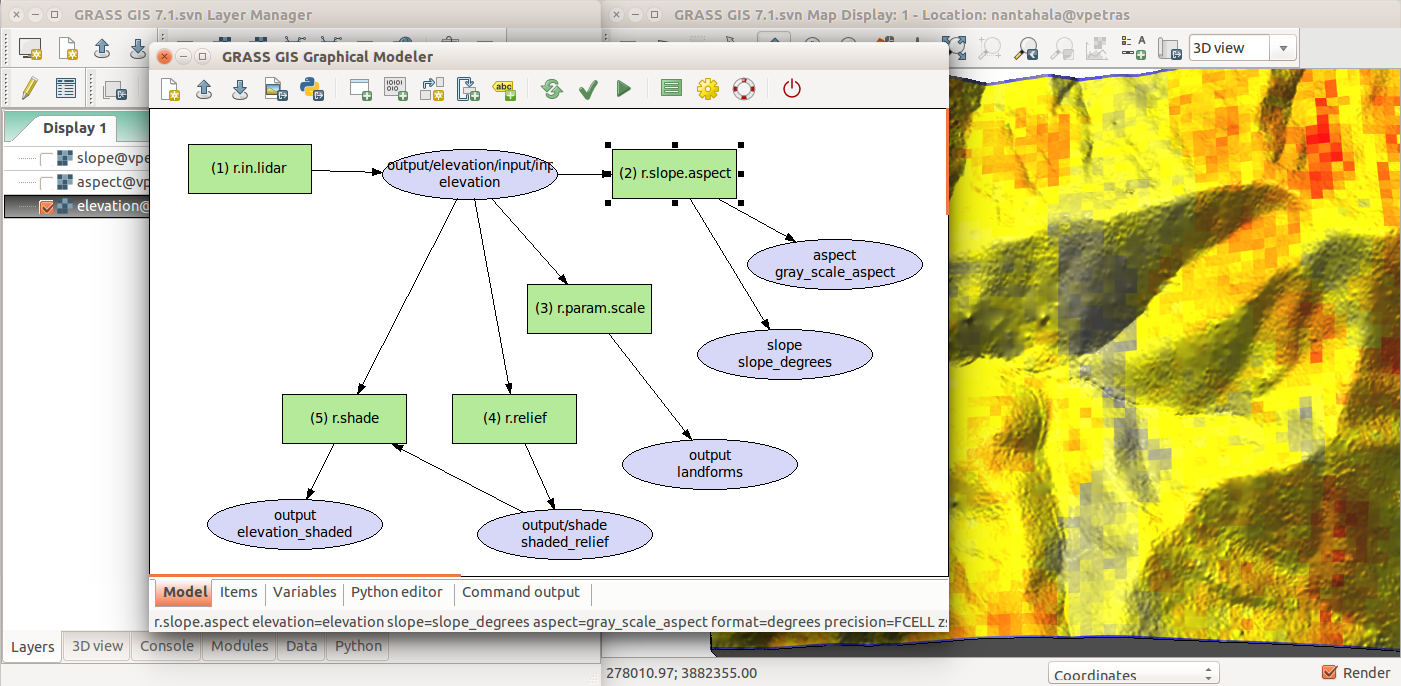
\includegraphics[width=0.9\textwidth]{grass/modeler}
\end{center}

\end{frame}


%%%%%%%%%%%%%%%%%%%%%%%%%%%%%%%%%%%%%%%%%%%%%%%%%%%%%%%%%%%%%%%%%%%%%
\begin{frame}{Points}

\begin{columns}
\begin{column}{0.3\textwidth}

\begin{itemize}
  \item collected by lidar
  \item generated by Structure from Motion (SfM) from UAV imagery
\end{itemize}

\end{column}
\begin{column}{0.65\textwidth}

\begin{center}
  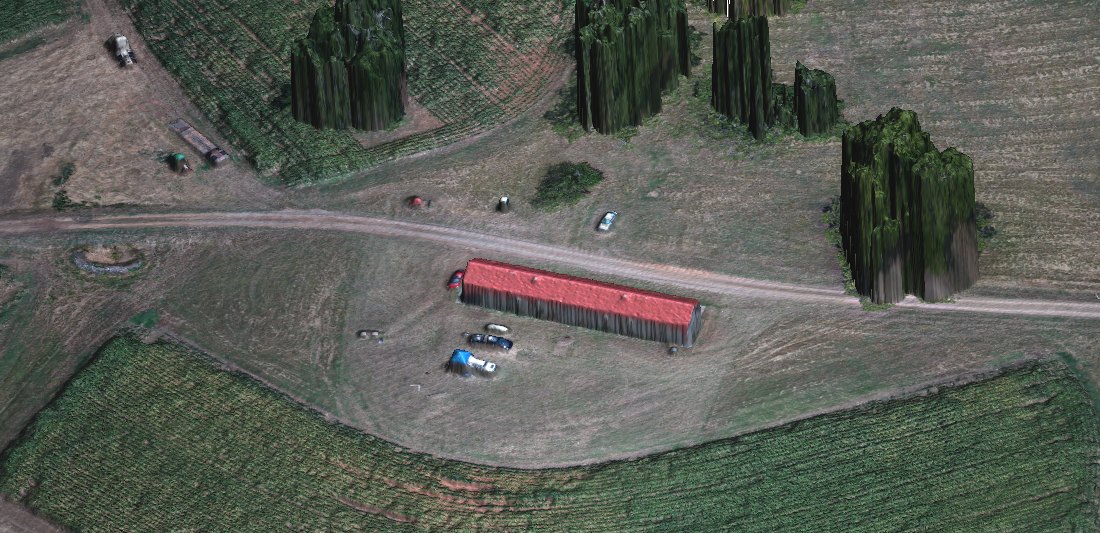
\includegraphics[width=\textwidth]{agisoft_detail}
  \\
  \tiny
  \textcolor{gray}{surface interpolated from points and visualized in GRASS GIS}
\end{center}

\end{column}
\end{columns}

\end{frame}


%%%%%%%%%%%%%%%%%%%%%%%%%%%%%%%%%%%%%%%%%%%%%%%%%%%%%%%%%%%%%%%%%%%%%
\begin{frame}{Workflow overview}

\includegraphics[width=\textwidth]%
    {grass/workflow}

\end{frame}


%%%%%%%%%%%%%%%%%%%%%%%%%%%%%%%%%%%%%%%%%%%%%%%%%%%%%%%%%%%%%%%%%%%%%
\begin{frame}{Surface interpolation}

\begin{columns}
\begin{column}{0.5\textwidth}

\begin{itemize}
  \item \gmodule{v.surf.idw}
  \begin{itemize}
    \item Inverse Distance squared Weighting
  \end{itemize}
  \item \gmodule{v.surf.bspline}
  \begin{itemize}
    \item Bicubic or bilinear Spline interpolation with Tykhonov regularization
  \end{itemize}
  \item \gmodule{v.surf.rst}
  \begin{itemize}
    \item Regularized Spline with Tension
    \item \gmodule{v.surf.rst.mp} (experimental)
    \begin{itemize}
      \item 2 millions of points in 11~minutes
    \end{itemize}
  \end{itemize}
\end{itemize}

\end{column}
\begin{column}{0.4\textwidth}

\begin{center}
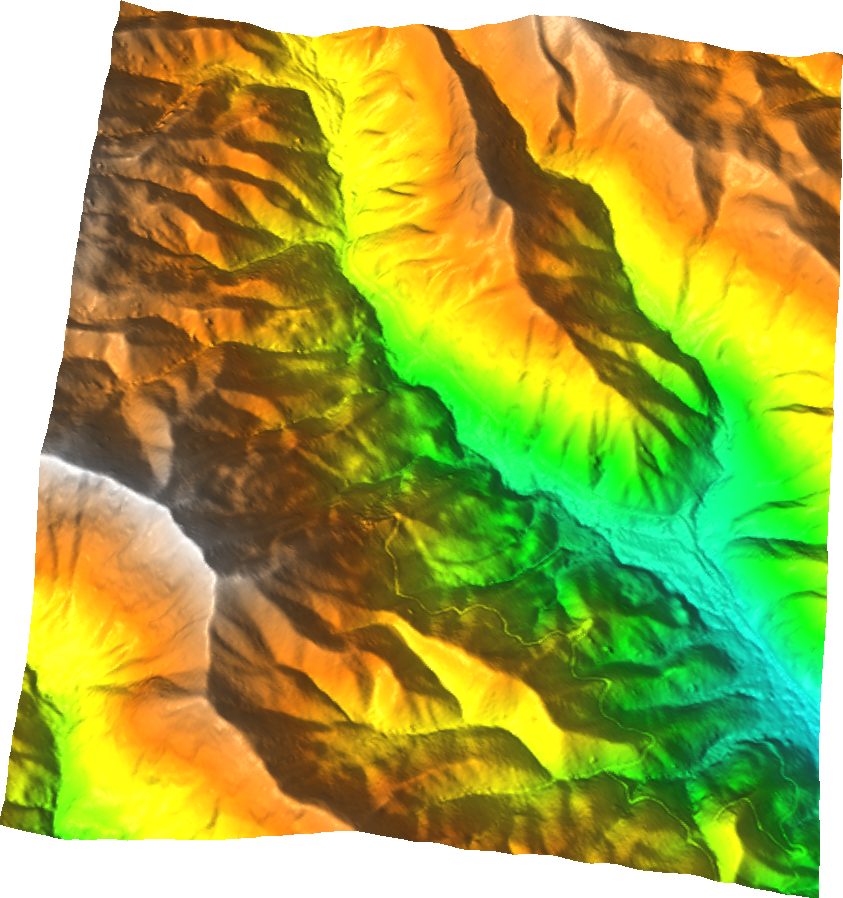
\includegraphics[width=\textwidth]{features/surface}
\end{center}

\end{column}
\end{columns}

\end{frame}


%%%%%%%%%%%%%%%%%%%%%%%%%%%%%%%%%%%%%%%%%%%%%%%%%%%%%%%%%%%%%%%%%%%%%
\begin{frame}{Import and decimation}

\begin{columns}
\begin{column}{0.58\textwidth}

\begin{itemize}
  \item \gmodule{v.in.lidar}
  \begin{itemize}
   \item libLAS
   \item LAS/LAZ to GRASS GIS native vector
    \item data stored in GRASS GIS database
  \end{itemize}
  \item interpolation, clustering, \ldots\ are costly
  \item often more points than we need
  \item decimation~$\approx$~thinning~$\approx$~sampling
  \begin{itemize}
    \item count-based decimation (skips points)
    \item grid-based experimental, others needed?
  \end{itemize}
\end{itemize}

\end{column}
\begin{column}{0.22\textwidth}

% TODO: UAV image

\begin{center}
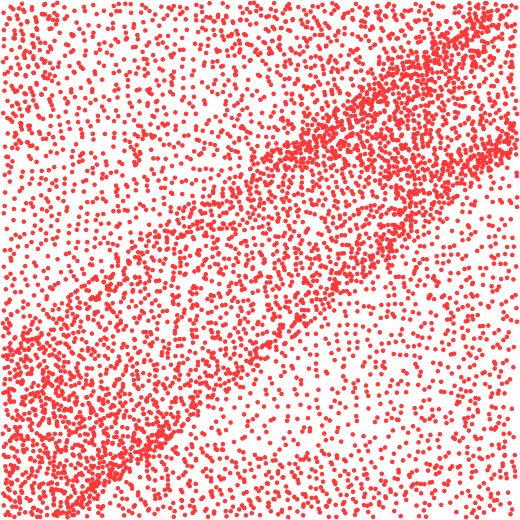
\includegraphics[width=\textwidth]{features/full}

\smallskip

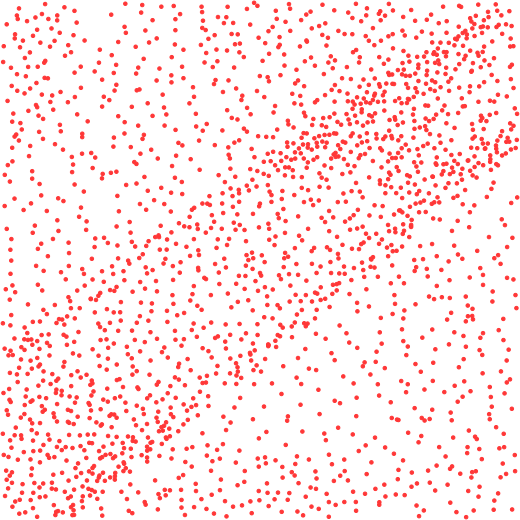
\includegraphics[width=\textwidth]{features/preserve}

\end{center}

\end{column}
\end{columns}

\end{frame}


%%%%%%%%%%%%%%%%%%%%%%%%%%%%%%%%%%%%%%%%%%%%%%%%%%%%%%%%%%%%%%%%%%%%%
\begin{frame}{Evaluating level of detail}

\begin{itemize}
  \item Local relief model (LRM)
  \item \amodule{r.local.relief} (micro-topography, features other than trend)
\end{itemize}

\begin{center}
  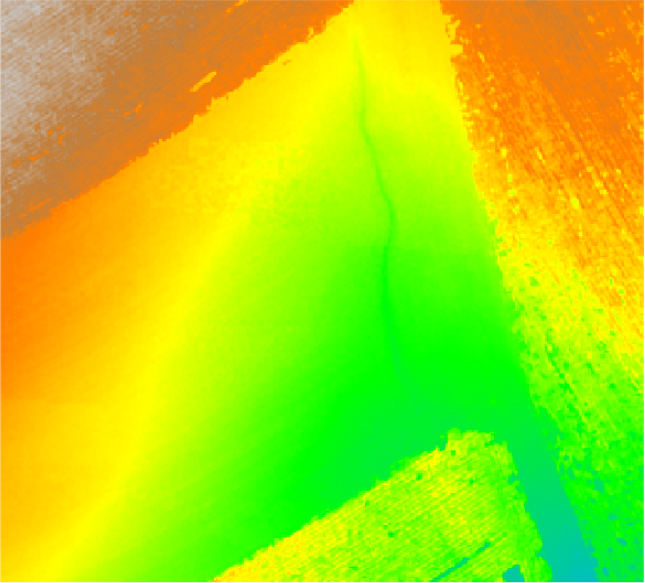
\includegraphics[width=0.4\textwidth]{vis/elevation}
  ~~
  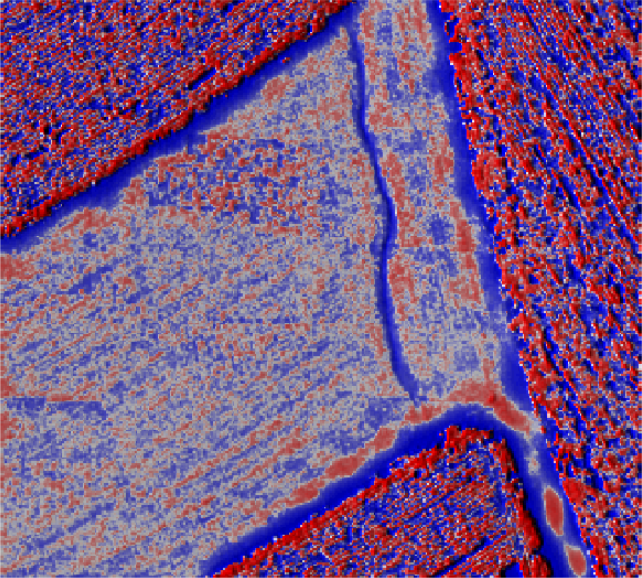
\includegraphics[width=0.4\textwidth]{vis/lrm}\\
  \footnotesize
  30-60cm wide, 30cm deep, 60m long gully (resolution 30cm)
  % 294 rows, 325 cols (88.2m x 97.5m)
\end{center}

\end{frame}


%%%%%%%%%%%%%%%%%%%%%%%%%%%%%%%%%%%%%%%%%%%%%%%%%%%%%%%%%%%%%%%%%%%%%
\begin{frame}{Influence of grid-based decimation resolution}

\newcommand{\imgsize}{0.23\textwidth}

\centering
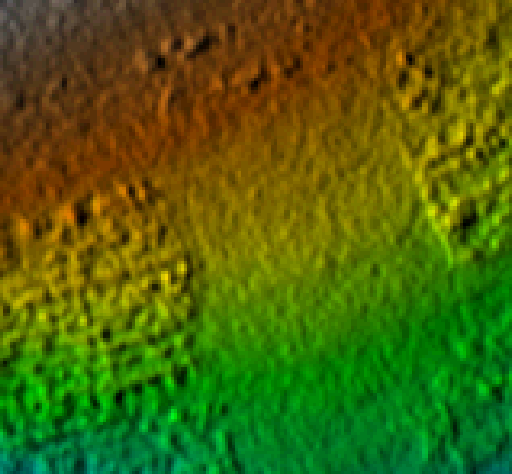
\includegraphics[width=\imgsize]{uav_grid_points_res_0_1_shaded_elevation}%
~%
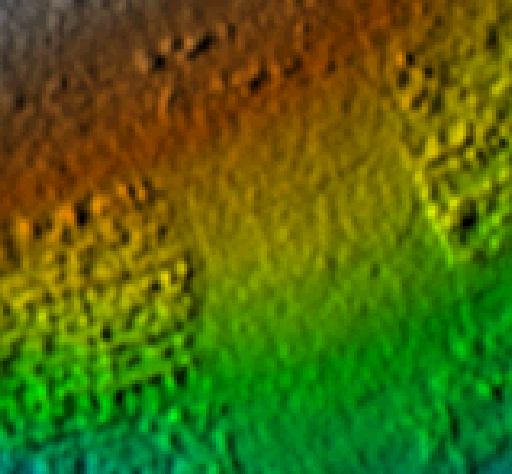
\includegraphics[width=\imgsize]{uav_grid_points_res_0_3_shaded_elevation}%
~%
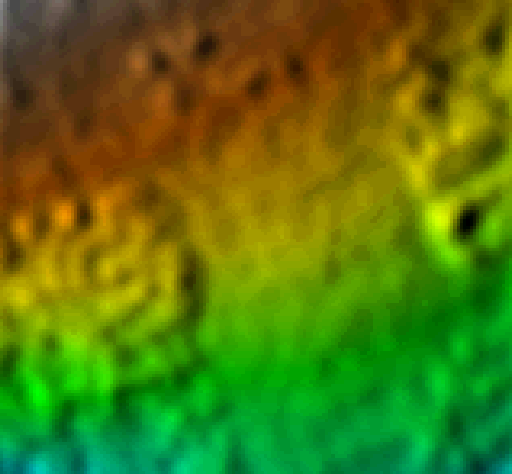
\includegraphics[width=\imgsize]{uav_grid_points_res_0_9_shaded_elevation}%
~%
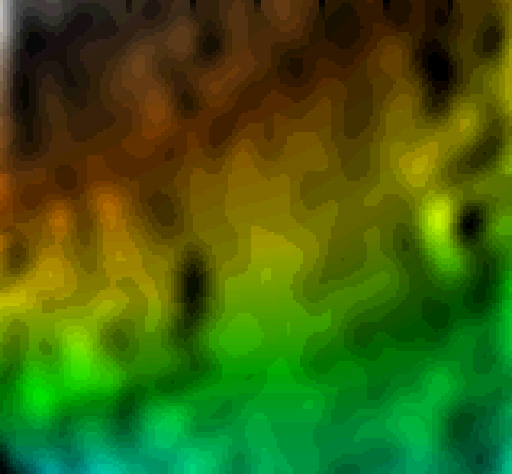
\includegraphics[width=\imgsize]{uav_grid_points_res_1_5_shaded_elevation}%

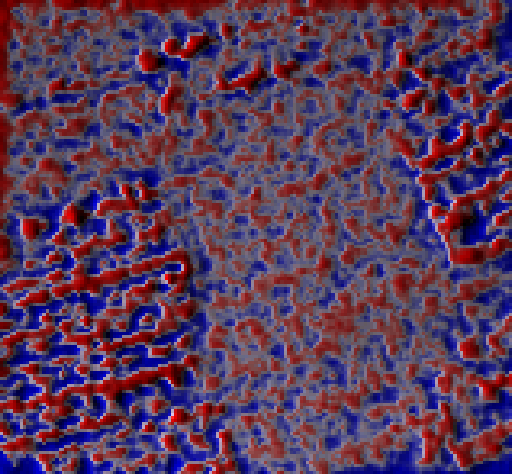
\includegraphics[width=\imgsize]{uav_grid_points_res_0_1_lrm_shaded}%
~%
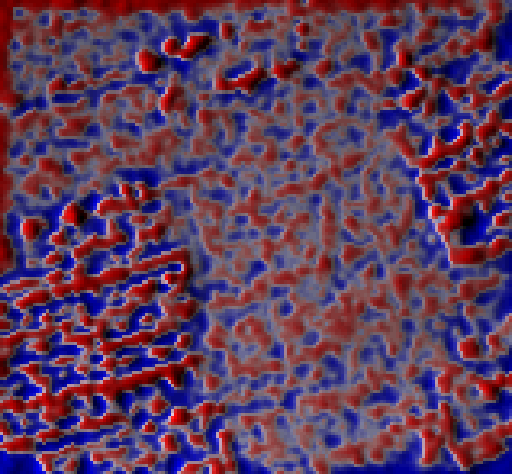
\includegraphics[width=\imgsize]{uav_grid_points_res_0_3_lrm_shaded}%
~%
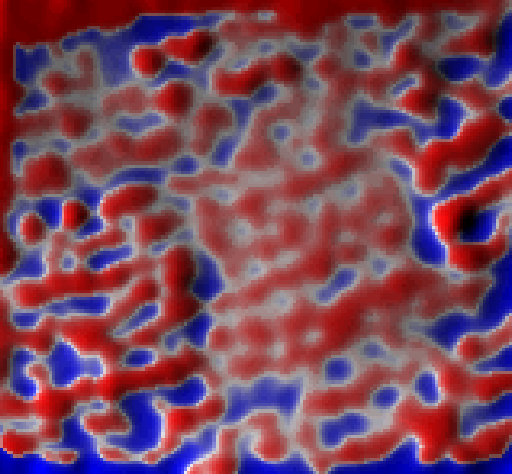
\includegraphics[width=\imgsize]{uav_grid_points_res_0_9_lrm_shaded}%
~%
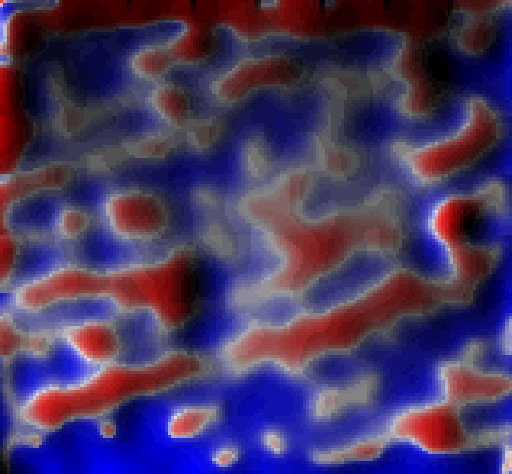
\includegraphics[width=\imgsize]{uav_grid_points_res_1_5_lrm_shaded}%

\newcommand{\captionfont}{\small}%
\makebox[\imgsize][c]{\captionfont grid size 0.1 m}%
~%
\makebox[\imgsize][c]{\captionfont grid size 0.3 m}%
~%
\makebox[\imgsize][c]{\captionfont grid size 0.9 m}%
~%
\makebox[\imgsize][c]{\captionfont grid size 1.5 m}%

\makebox[\imgsize][c]{\captionfont 0 \%}%
~%
\makebox[\imgsize][c]{\captionfont 81 \%}%
~%
\makebox[\imgsize][c]{\captionfont 98 \%}%
~%
\makebox[\imgsize][c]{\captionfont 99 \%}%

\textcolor{gray}{
\tiny
test data (not used in the study)
}

\end{frame}


%%%%%%%%%%%%%%%%%%%%%%%%%%%%%%%%%%%%%%%%%%%%%%%%%%%%%%%%%%%%%%%%%%%%%
\begin{frame}{Decimating UAV/SfM point cloud}

\begin{center}

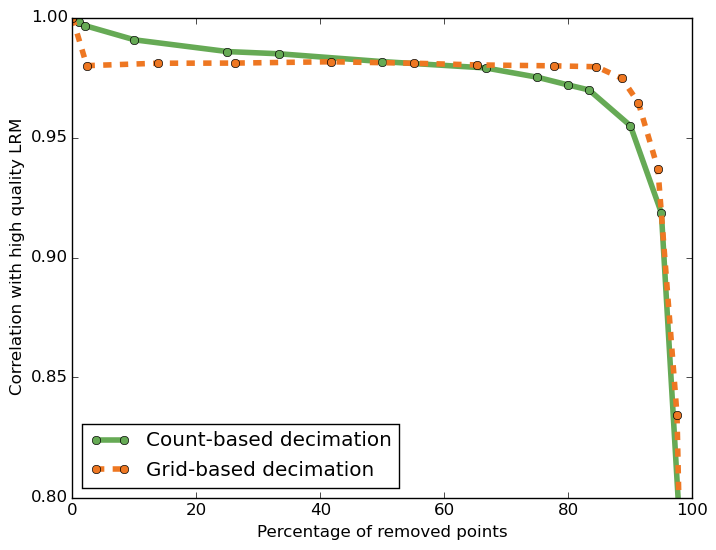
\includegraphics[width=0.7\textwidth]{decimation/lrm_grid_count_uav}

\end{center}

grid-based decimation may give slightly better results
\textcolor{gray}{
\tiny
\\
at resolution 0.5~m for all raster calculations,
72~point per 1~m$^2$
}

\end{frame}


%%%%%%%%%%%%%%%%%%%%%%%%%%%%%%%%%%%%%%%%%%%%%%%%%%%%%%%%%%%%%%%%%%%%%
\begin{frame}{Decimating lidar point cloud}

\begin{center}
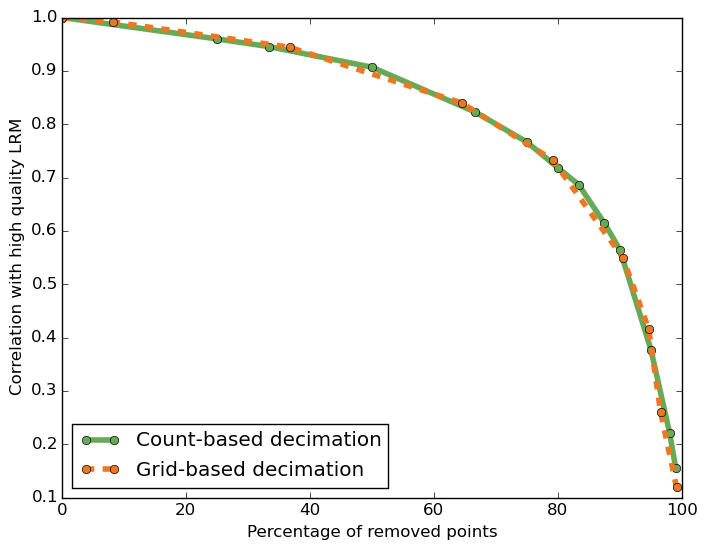
\includegraphics[width=0.7\textwidth]{decimation/lrm_grid_count_lidar}

\end{center}

fast count-based decimation as good as more advanced grid-based decimation
\textcolor{gray}{
\tiny
at resolution 0.5~m for all raster calculations,
1~point per 1~m$^2$
}

\end{frame}


%%%%%%%%%%%%%%%%%%%%%%%%%%%%%%%%%%%%%%%%%%%%%%%%%%%%%%%%%%%%%%%%%%%%%
\begin{frame}{Binning points to raster}

\begin{columns}
\begin{column}{0.4\textwidth}

 \begin{itemize}
  \item \gmodule{r.in.lidar}
  \item import and analysis
  \item statistics of point counts, height and intensity
  \begin{itemize}
    \item n, min, max, sum
    \item mean, range, skewness, \ldots
  \end{itemize}
\end{itemize}

\end{column}
\begin{column}{0.45\textwidth}

\begin{center}
  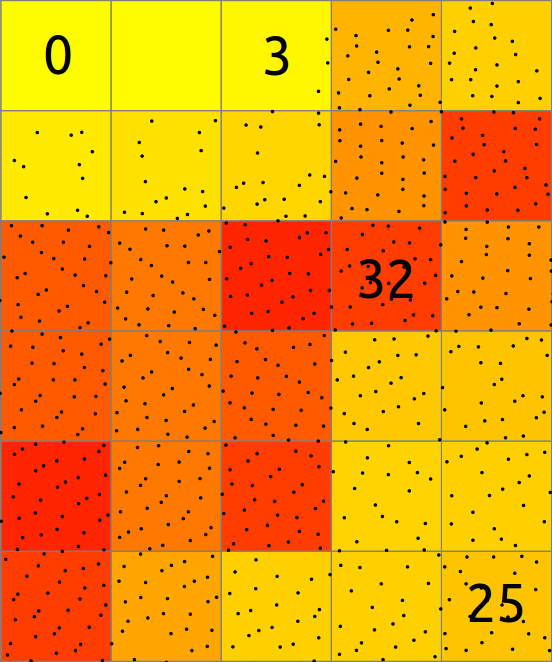
\includegraphics[width=0.75\textwidth]{features/binning_count}
\end{center}

\end{column}
\end{columns}

\end{frame}


%%%%%%%%%%%%%%%%%%%%%%%%%%%%%%%%%%%%%%%%%%%%%%%%%%%%%%%%%%%%%%%%%%%%%
\begin{frame}{Raster processing}

% $ cd dist
% $ cd bin
% $ ls r.* | wc -l
% 143
% $ ls i.* | wc -l
% 38
% $ cd ../scripts
% $ ls r.* | wc -l
% 20
% $ ls i.* | wc -l
% 7
% $ ls t.rast.* | wc -l
% 20

% $ cd dist
% $ ls bin/r.* scripts/r.* | wc -l
% 163
% $ ls bin/i.* scripts/i.* | wc -l
% 45
% $ ls scripts/t.rast.* | wc -l
% 20


\begin{columns}
\begin{column}{0.5\textwidth}

\begin{itemize}
  \item many algorithms are raster-based
  \begin{itemize}
    \item 163 raster modules
    \item 45 imagery modules
    \item 20 spatio-temporal raster modules
  \end{itemize}
  \item example:
  \begin{enumerate}
    \item count of ground points
    \item count of non-ground points
    \item used as image bands
    \item segmentation using \gmodule{i.segment}
  \end{enumerate}
\end{itemize}

\end{column}
\begin{column}{0.45\textwidth}

\begin{center}
  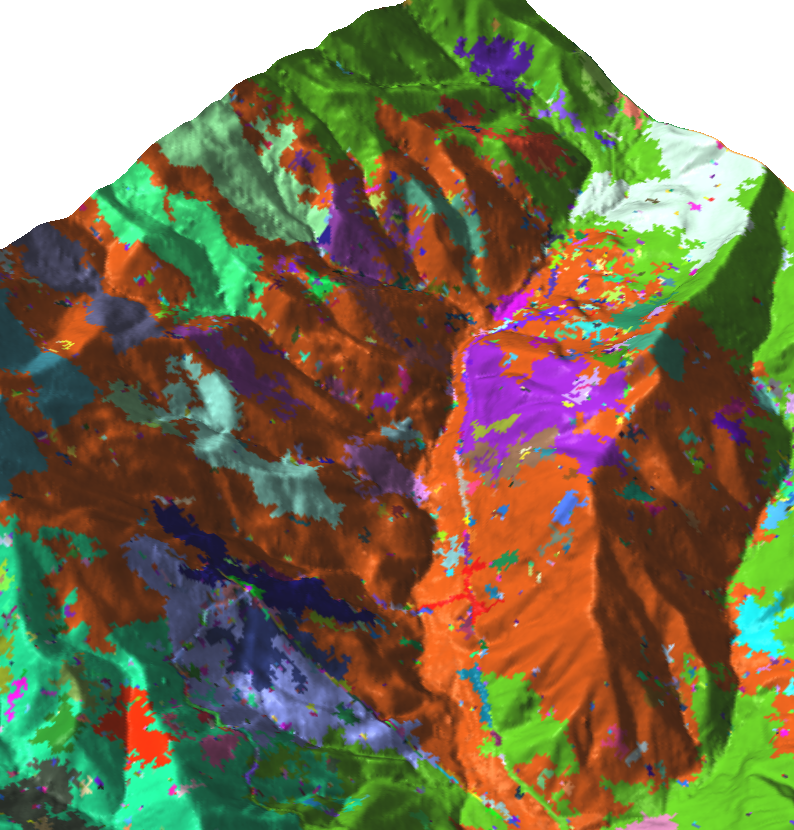
\includegraphics[width=0.9\textwidth]{grass/segment_on_counts}
\end{center}

\end{column}
\end{columns}

\end{frame}

%%%%%%%%%%%%%%%%%%%%%%%%%%%%%%%%%%%%%%%%%%%%%%%%%%%%%%%%%%%%%%%%%%%%%
\begin{frame}{3D raster}

\begin{columns}
\begin{column}{0.38\textwidth}

\begin{itemize}
  \item same principles as in~2D
  \begin{itemize}
  \item e.g. 3D raster map algebra
  \end{itemize}
  \item challenging to visualize
\end{itemize}

\end{column}
\begin{column}{0.5\textwidth}

\begin{center}
  \includegraphics<1>[width=\textwidth]{grass/raster_3d_cube}
  \includegraphics<2>[width=\textwidth]{grass/raster_3d_slices}
\end{center}

\end{column}
\end{columns}

% vis also possible using Tangible Landscape

\end{frame}


%%%%%%%%%%%%%%%%%%%%%%%%%%%%%%%%%%%%%%%%%%%%%%%%%%%%%%%%%%%%%%%%%%%%%
\begin{frame}{Binning points to 3D raster}

\begin{columns}
\begin{column}{0.28\textwidth}

\begin{itemize}
  \item \gmodule{r3.in.lidar}
  \item count per 3D cell relative to the count per vertical column
\end{itemize}

\end{column}
\begin{column}{0.7\textwidth}

\begin{center}
  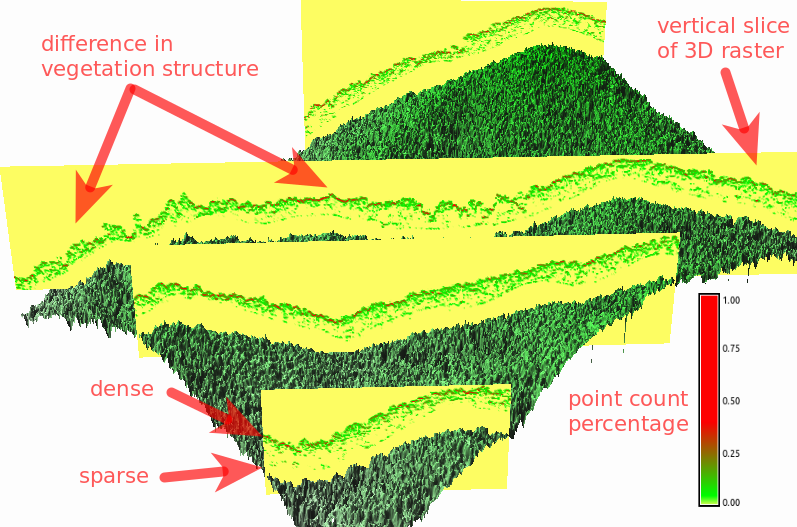
\includegraphics[width=\textwidth]{grass/red_green_3d_labels}
\end{center}

\end{column}
\end{columns}

\end{frame}

%%%%%%%%%%%%%%%%%%%%%%%%%%%%%%%%%%%%%%%%%%%%%%%%%%%%%%%%%%%%%%%%%%%%%
\begin{frame}{Point heights reduced to surface}

\begin{center}
  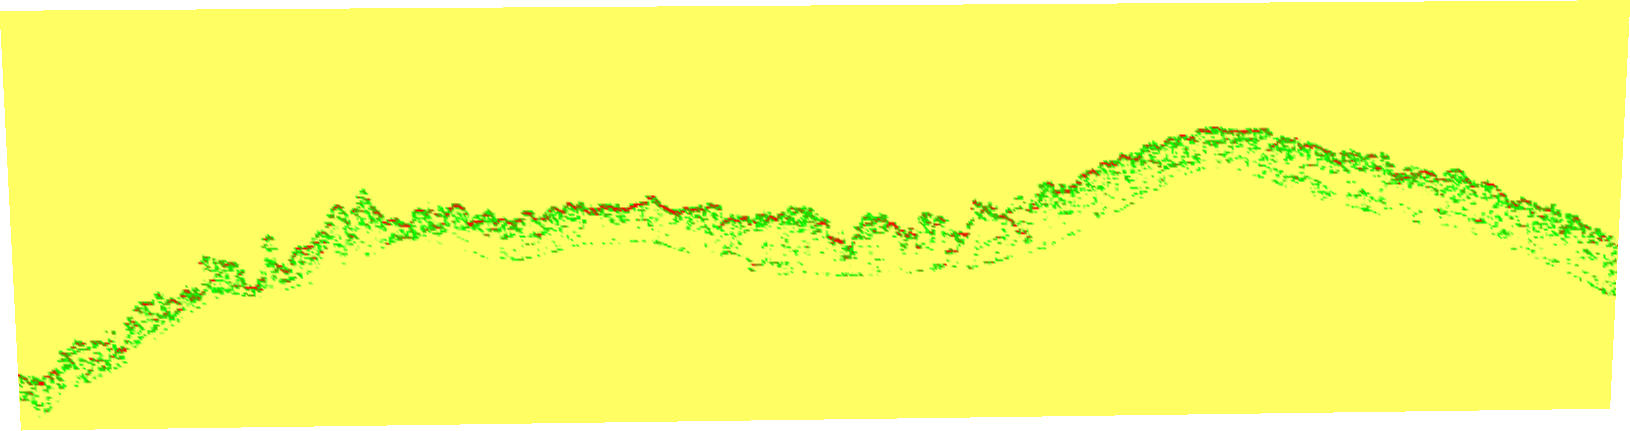
\includegraphics[width=0.8\textwidth]{features/rast3_real}

  \bigskip

  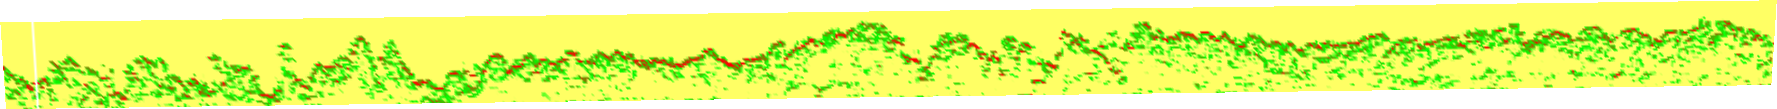
\includegraphics[width=0.8\textwidth]{features/rast3_base}
\end{center}

\begin{itemize}
  \item \gmodule{r3.in.lidar}, option \textit{base\_raster}
  \item height reduced by 2D raster values
\end{itemize}

\end{frame}


%%%%%%%%%%%%%%%%%%%%%%%%%%%%%%%%%%%%%%%%%%%%%%%%%%%%%%%%%%%%%%%%%%%%%
\begin{frame}{Ground detection}

\begin{columns}
\begin{column}{0.35\textwidth}

\begin{itemize}
\item \gmodule{v.lidar.edgedetection}, \gmodule{v.lidar.growing}, \gmodule{v.lidar.correction}
\begin{itemize}
  \item \tiny by Brovelli, Cannata, Antolin \& Moreno
\end{itemize}

\item \amodule{v.lidar.mcc}
\begin{itemize}
  \item \tiny multiscale curvature based classification algorithm
  \item \tiny by Blumentrath, according to Evans \& Hudak
\end{itemize}

\item PDAL filters.ground
\begin{itemize}
  \item \tiny currently in v.in.pdal
  \item \tiny progressive morphological filter by Zhang
  \item \tiny provided by PCL
\end{itemize}

\end{itemize}

\end{column}
\begin{column}{0.64\textwidth}

\begin{center}
  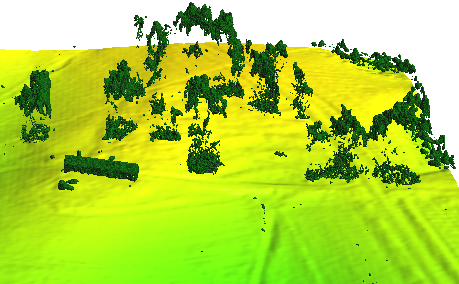
\includegraphics[width=\textwidth]{grass/mcc_default_smaller}
\end{center}

\end{column}
\end{columns}

\end{frame}


%%%%%%%%%%%%%%%%%%%%%%%%%%%%%%%%%%%%%%%%%%%%%%%%%%%%%%%%%%%%%%%%%%%%%
\begin{frame}{Integration with PDAL}

\begin{columns}
\begin{column}{0.5\textwidth}

\begin{block}{PDAL}
 \begin{itemize}
  \item Point Data Abstraction Library
  \item format conversions
  \item processing, filtering
 \end{itemize}
\end{block}

\end{column}
\begin{column}{0.25\textwidth}

\begin{center}
  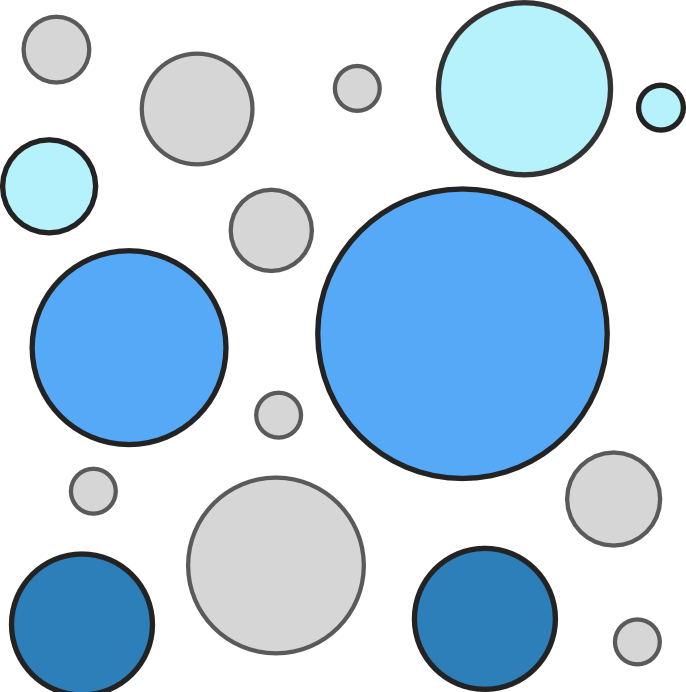
\includegraphics[width=\textwidth]{logos/pdal_bubbles}\\
  
\includegraphics[width=\textwidth]{logos/pdal_text}
\end{center}

\end{column}
\end{columns}

\end{frame}


%%%%%%%%%%%%%%%%%%%%%%%%%%%%%%%%%%%%%%%%%%%%%%%%%%%%%%%%%%%%%%%%%%%%%
\begin{frame}{Using other open source projects}

\begin{columns}
\begin{column}{0.5\textwidth}

\begin{block}{\module{r.in.kinect}}
 \begin{itemize}
  \item scans using Kinect
  \item OpenKinect libfreenect2
  \item Point Cloud Library (PCL)
  \item GRASS GIS libraries
 \end{itemize}
\end{block}

% inner columns
\begin{columns}
\begin{column}{0.6\textwidth}
\small

used in Tangible~Landscape

\end{column}
\begin{column}{0.2\textwidth}


\includegraphics[width=\textwidth]{logos/tangible_landscape}

\end{column}
\end{columns}
% end of inner columns

\end{column}
\begin{column}{0.45\textwidth}

\begin{center}
  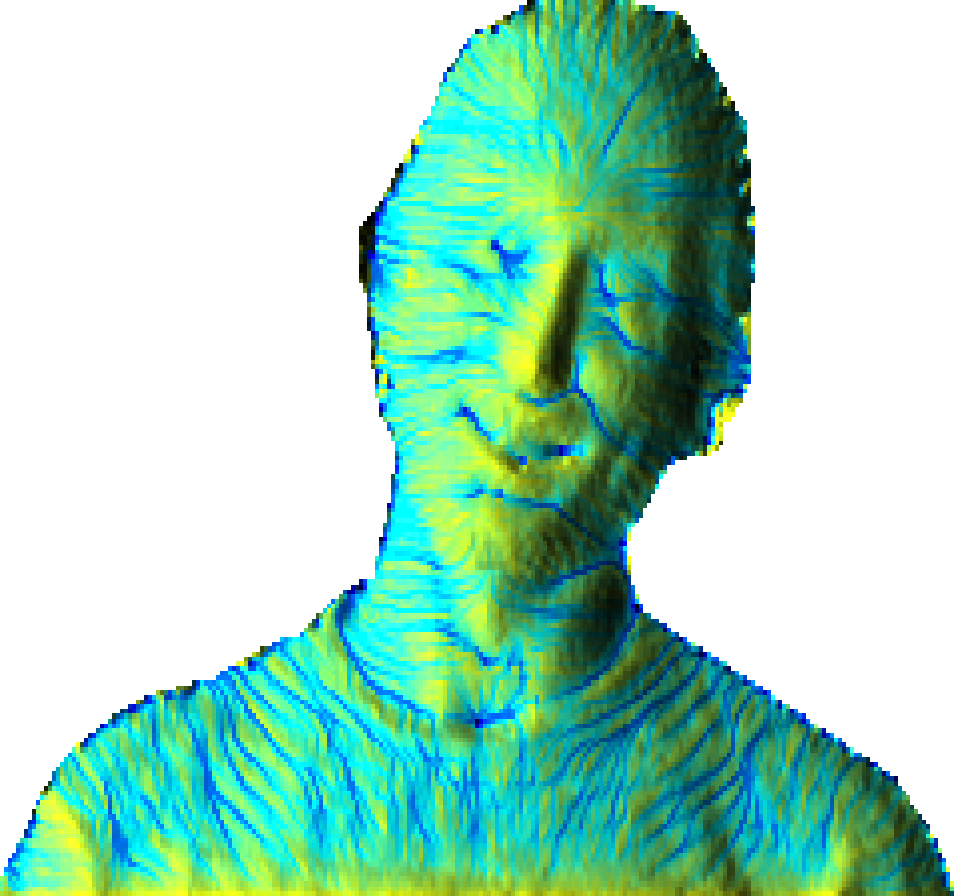
\includegraphics[width=\textwidth]{tangible/face}
\end{center}

\end{column}
\end{columns}

\end{frame}


%%%%%%%%%%%%%%%%%%%%%%%%%%%%%%%%%%%%%%%%%%%%%%%%%%%%%%%%%%%%%%%%%%%%%
\begin{frame}{}

% logo at the bottom can be moved down
\vspace*{0.05\textheight}

\begin{block}{Summary}
 \begin{itemize}
  \item decimation or \emph{rasterize early} approach for large point clouds
  \item 3D rasters
  \item PDAL integration
 \end{itemize}
\end{block}

\bigskip
\centering

\begin{tabular}{clc}
\begin{minipage}{0.16\textwidth}

\includegraphics[width=\textwidth]{logos/grass_gis}
\end{minipage}
&
\begin{minipage}{0.5\textwidth}
\footnotesize
\href{https://grass.osgeo.org/download/}{%
Get GRASS GIS 7.3 development version at\\
\texttt{grass.osgeo.org/download}%
}

\bigskip

{
\footnotesize
\href{https://lists.osgeo.org/listinfo/grass-user}{GRASS user mailing list}\\
\href{https://lists.osgeo.org/listinfo/grass-user}{\texttt{lists.osgeo.org/listinfo/grass-user}}
}

\bigskip

{
\footnotesize
Paper and slides available at\\
\href{http://wenzeslaus.github.io/grass-lidar-talks/}%
  {\texttt{wenzeslaus.github.io/grass-lidar-talks}}
}
\end{minipage}
&
\begin{minipage}{0.2\textwidth}

\includegraphics[width=\textwidth]{talks_qr}
\end{minipage}
\end{tabular}

\end{frame}

% don't count the backup and ack slides
\backupbegin

%%%%%%%%%%%%%%%%%%%%%%%%%%%%%%%%%%%%%%%%%%%%%%%%%%%%%%%%%%%%%%%%%%%%%
\begin{frame}{Acknowledgements}

\begin{columns}
\begin{column}{0.6\textwidth}

\begin{block}{Software}
Presented functionality is work done by Vaclav Petras, Markus Metz, and the GRASS development team.

\bigskip

Thanks to users for feedback and testing, especially to
Doug Newcomb, Markus Neteler, Laura Belica, and William Hargrove.
\end{block}

\end{column}
\begin{column}{0.3\textwidth}

\begin{center}
  
\includegraphics[width=\textwidth]{logos/grass_gis}
\end{center}

\end{column}
\end{columns}

\end{frame}


%%%%%%%%%%%%%%%%%%%%%%%%%%%%%%%%%%%%%%%%%%%%%%%%%%%%%%%%%%%%%%%%%%%%%
\begin{frame}{Acknowledgements}

\begin{columns}
\begin{column}{0.48\textwidth}

\begin{block}{Datasets}
\footnotesize
Lidar and UAV Structure from Motion (SfM) data for
\href{http://ncsu-osgeorel.github.io/uav-lidar-analytics-course/}%
  {GIS595/MEA792: UAV/lidar Data Analytics} course

\smallskip

Nantahala NF, NC: Forest Leaf Structure, Terrain and Hydrophysiology.
% Lidar data acquisition and processing completed
% by the National Center for Airborne Laser Mapping (\href{http://www.ncalm.org}{NCALM}).
% NCALM funding provided by NSF's Division of Earth Sciences, Instrumentation and Facilities Program.
% EAR-1043051.
Obtained from \href{http://www.opentopography.org/}{OpenTopography}.
\url{http://dx.doi.org/10.5069/G9HT2M76}
\end{block}

\end{column}
\begin{column}{0.47\textwidth}

\begin{center}
  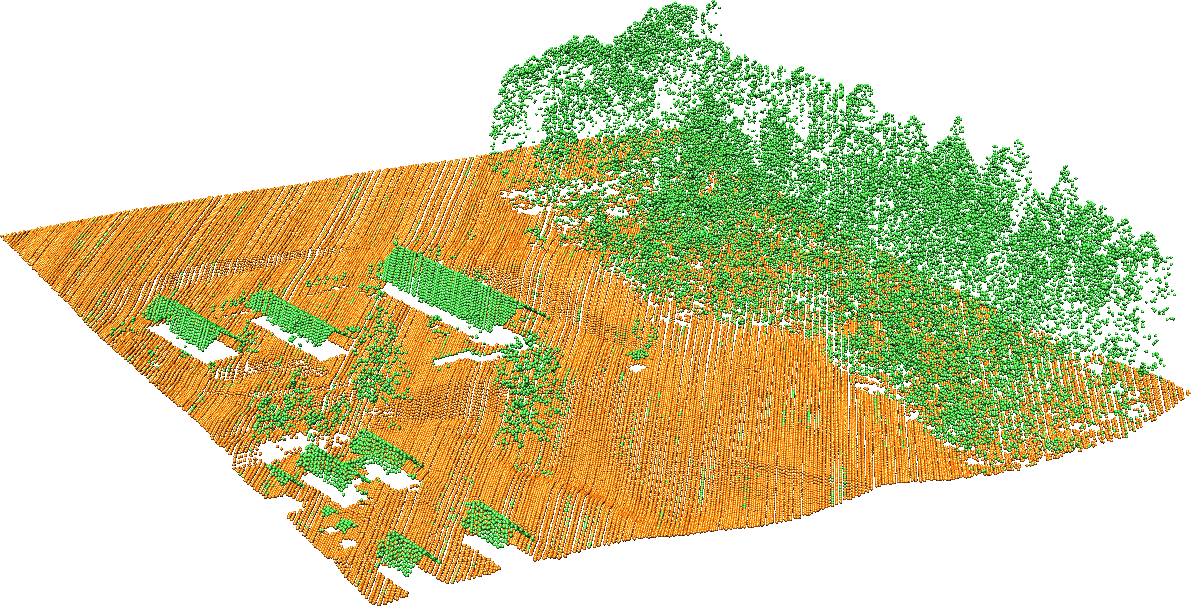
\includegraphics[width=\textwidth]{lidar_secref_3d}
\end{center}

\end{column}
\end{columns}

\end{frame}

%%%%%%%%%%%%%%%%%%%%%%%%%%%%%%%%%%%%%%%%%%%%%%%%%%%%%%%%%%%%%%%%%%%%%
\begin{frame}{Acknowledgements}

\begin{block}{Presentation software}
\Huge
\textrm{Slides were created in \LaTeX{} using the~\textsc{beamer} \textit{class}.}
% all lowercase, sc and it taken from the beamer user guide
\end{block}

\end{frame}

\backupend

\end{document}
